\documentclass[aspectratio=169]{beamer}
\usepackage{bookmark}
\usepackage{amsmath}
\usepackage{lifa}
\usepackage[style=ieee]{biblatex}
\setbeamertemplate{bibliography item}{\insertbiblabel}
\addbibresource{bibliography.bib}

\title{Adesão Celular}
\subtitle{A Base da Organização Tecidual}
\author{Gustavo O. Rosa}
\institute{Laboratório de Inovação em Física Aplicada}
% \date{\today}

\begin{document}
%% Página de título
%% Remova '[plain]' se precisar de um rodapé
\begin{frame}[plain]
    \titlepage
\end{frame}


% %% Página de Sumário
% {
% \begin{frame}
%     \frametitle{Sumário}
%     \tableofcontents
% \end{frame}
% }


\section{Introdução Biológica}

\begin{frame}{Importância da Ligação Celular}
    \begin{itemize}
        \item \textbf{Desenvolvimento de Órgãos e Manutenção Tecidual}: 
        Garante a coesão e integridade dos tecidos, formando a estrutura complexa dos organismos 
        multicelulares
        \item \textbf{Migração e Sinalização Celular}: Permite que as células se movam de forma
        coordenada e respondam a sinais do seu microambiente, crucial em processos como o 
        desenvolvimento embrionário e a cicatrização de feridas
        \item \textbf{Resposta Imune e Inflamação}: Essencial para a localização e movimentação de 
        células imunes para locais de infecção ou dano
    \end{itemize}
\end{frame}

\begin{frame}{Tipos de Ligação}
    As ligações devem ser não-covalentes para manter a dinâmica das células, existem diversas moléculas responsáveis, entre elas:
    \begin{itemize}
        \item \textbf{Caderinas}
        \item Grupo Ig
        \item \textbf{Integrinas}
        \item Selectinas 
        \item Mucinas
    \end{itemize}
    Essas ligações tem dois grandes grupos: \textbf{célula-célula} e \textbf{célula-matriz}
\end{frame}

\begin{frame}{Tipos de Ligação}
    \begin{figure}\label{fig:ligacao_geral}
        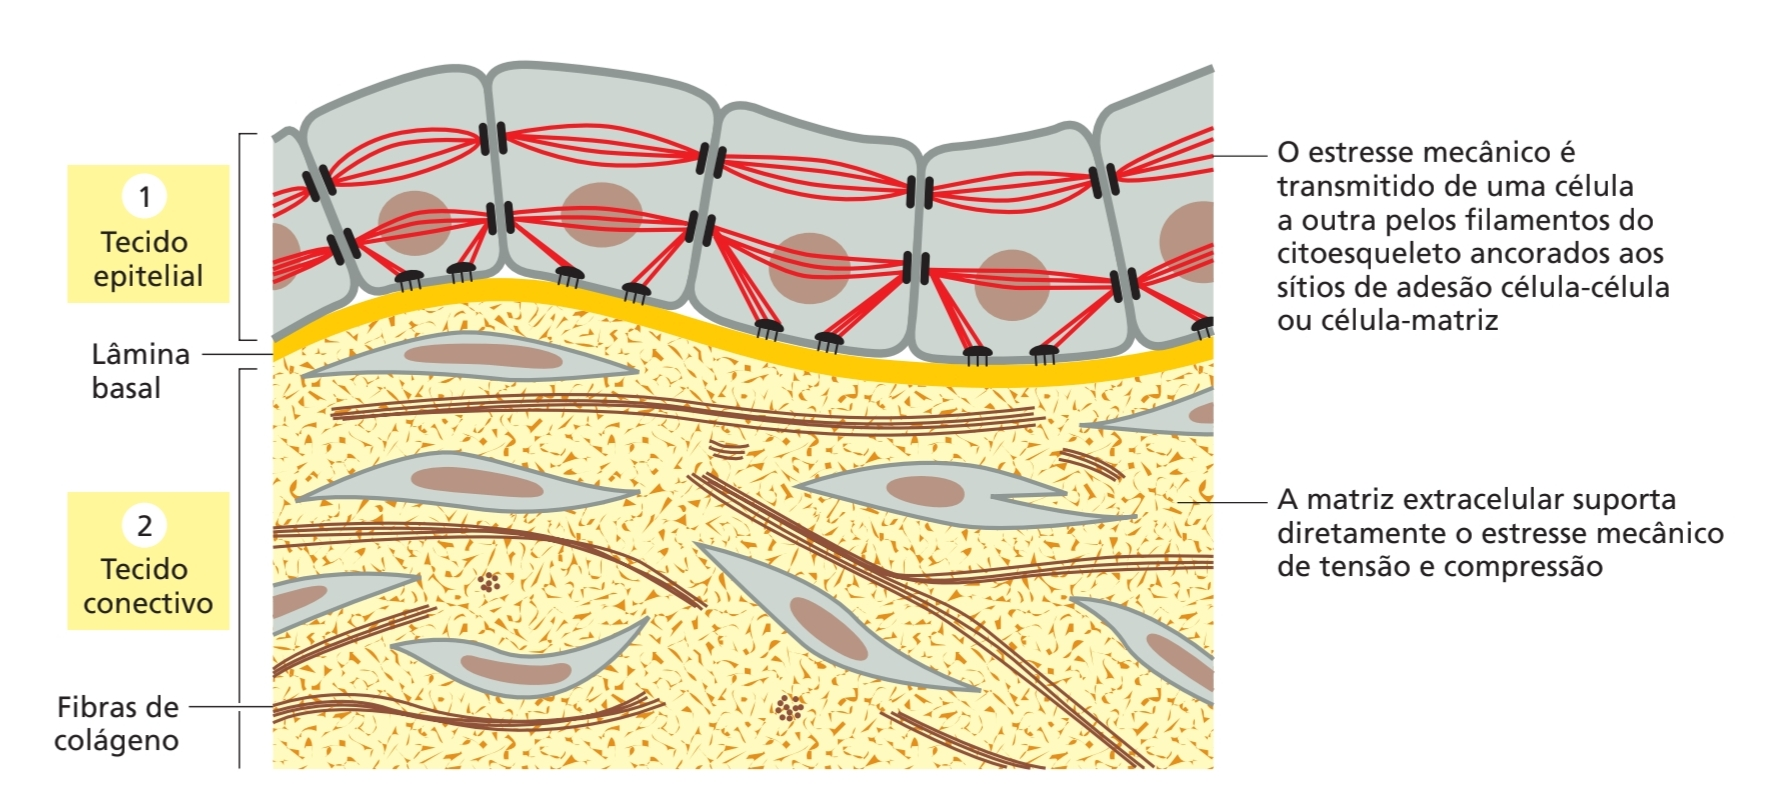
\includegraphics[width=0.9\textwidth]{img/bio/tipos_ligação.jpg}
        \caption{Imagem representativa dos tipos de ligação célula-célula e célula-matriz}
    \end{figure}
\end{frame}


\begin{frame}{Caderinas}
    \begin{columns}[c, onlytextwidth]
        \column{0.5\textwidth}
            \begin{itemize}
               \item As caderinas são responsáveis pelas ligações \textbf{célula-célula}
               \item A sua função é estritamente dependente de \textbf{íons cálcio}
               \item Processo dinâmico de ligação e dissociação
            \end{itemize}
        
        \column{0.5\textwidth}
            \begin{figure}\label{fig:caderinas}
                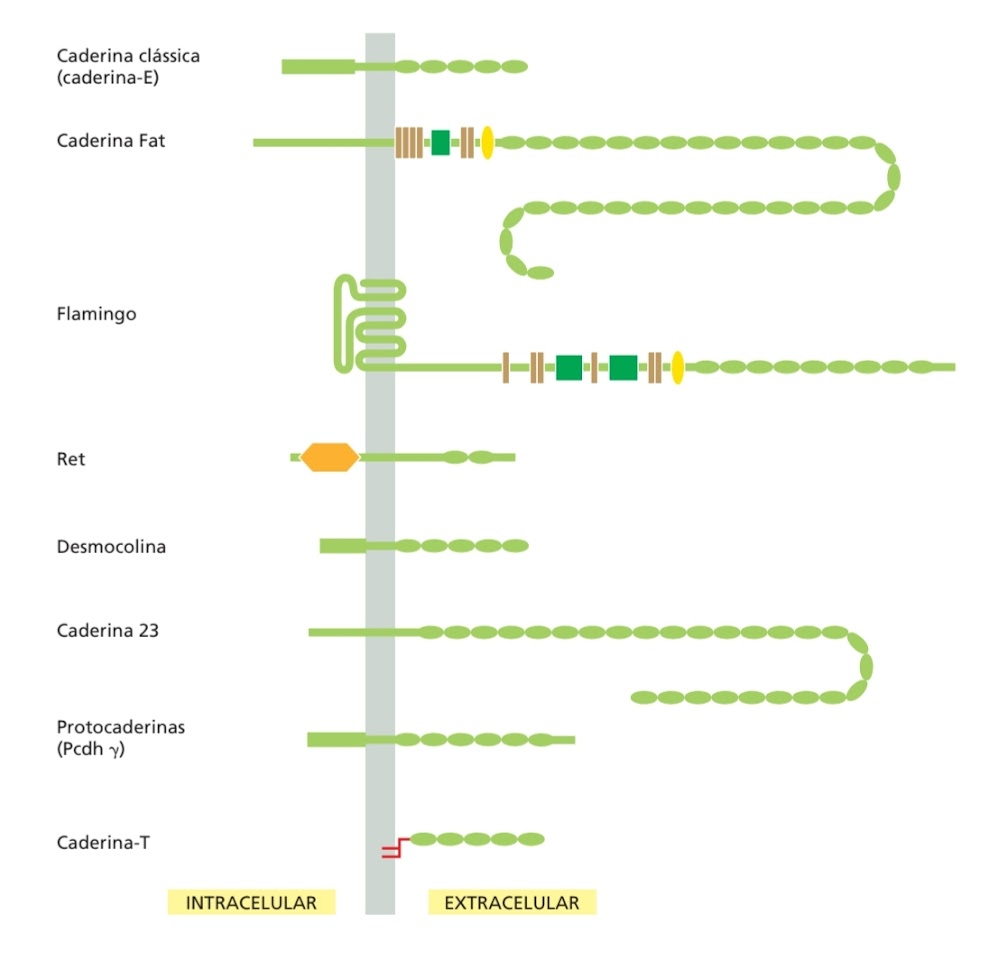
\includegraphics[width=0.9\textwidth]{img/bio/caderinas.jpg}
                \caption{Diferentes tipos de caderinas}
            \end{figure}
    \end{columns}
\end{frame}

\begin{frame}{Caderinas}
    \begin{figure}
        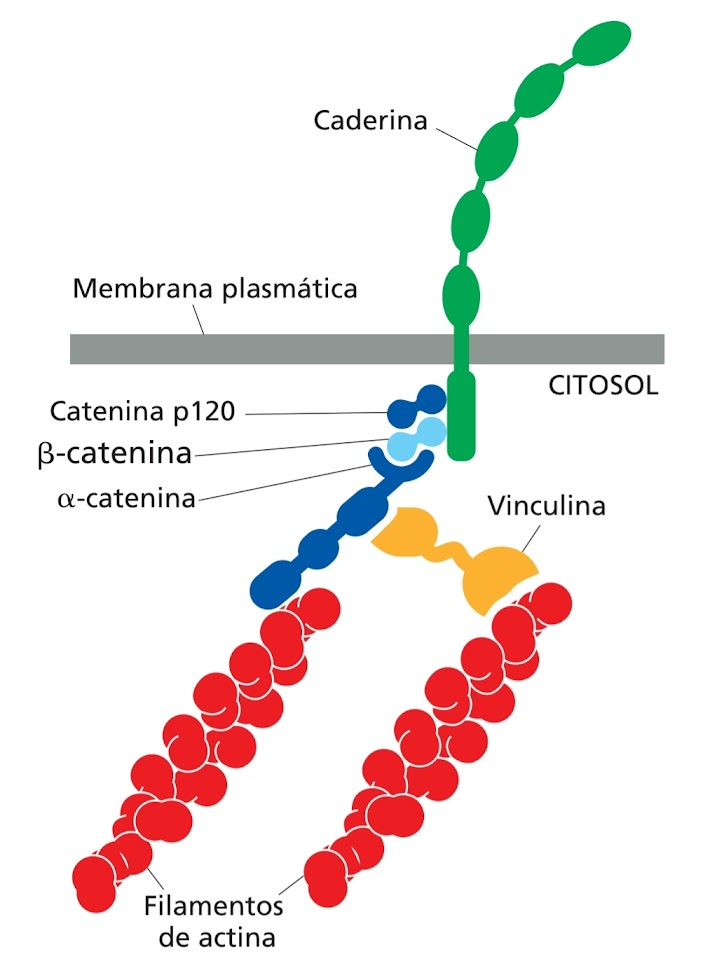
\includegraphics[width=0.32\textwidth]{img/bio/close_caderina.jpg}
        \caption{Visão geral da caderina}
    \end{figure}
\end{frame}

\begin{frame}{Outras ligações}
    \begin{columns}[t, onlytextwidth]
        \column{0.5 \textwidth}
            \begin{itemize}
                \item A \textbf{superfamília IG} liga em proteínas, como fibronectina, lamina e 
                colágeno e se ligam de forma homofílica ou heterofílica
                \item \textbf{Selectinas} se ligam com as \textbf{mucinas} em regiões com carboidratos
                e são responsáveis pela ligação incial de leucócitos em células endoteliais 
            \end{itemize}    

        \column{0.5\textwidth}
            \begin{figure}\label{fig:hetero_homo}
                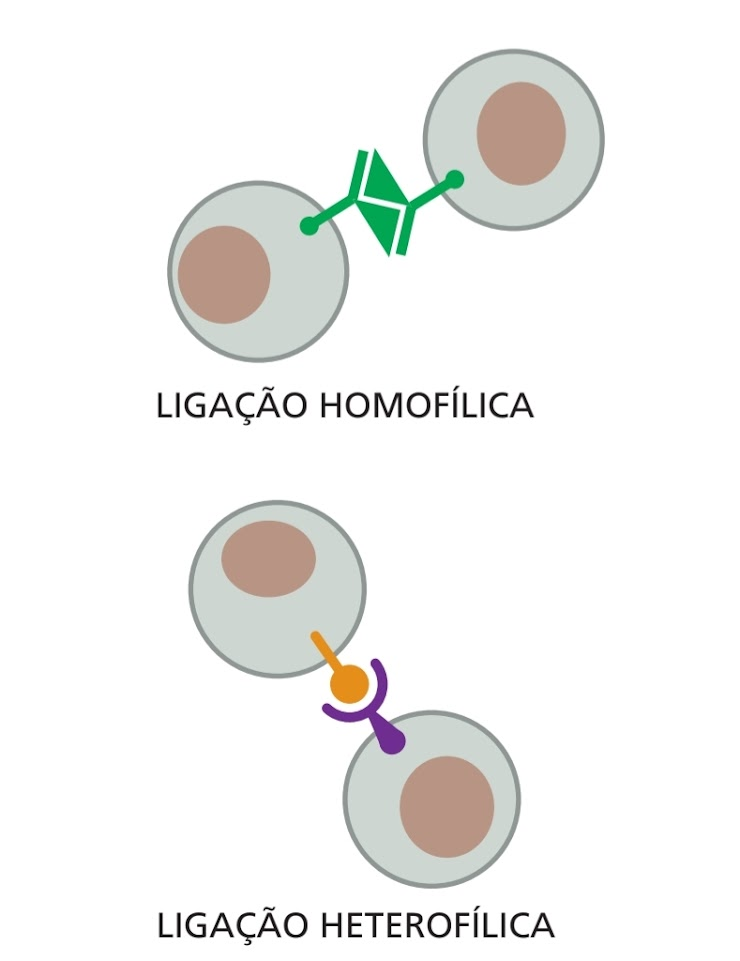
\includegraphics[width=0.6\textwidth]{img/bio/hetero_homo_bonds.jpg}
                \caption{Ligações heterofílica e homofílica}
            \end{figure}
    \end{columns}
\end{frame}

\begin{frame}{Ligações Célula-Célula}
    \begin{figure}
        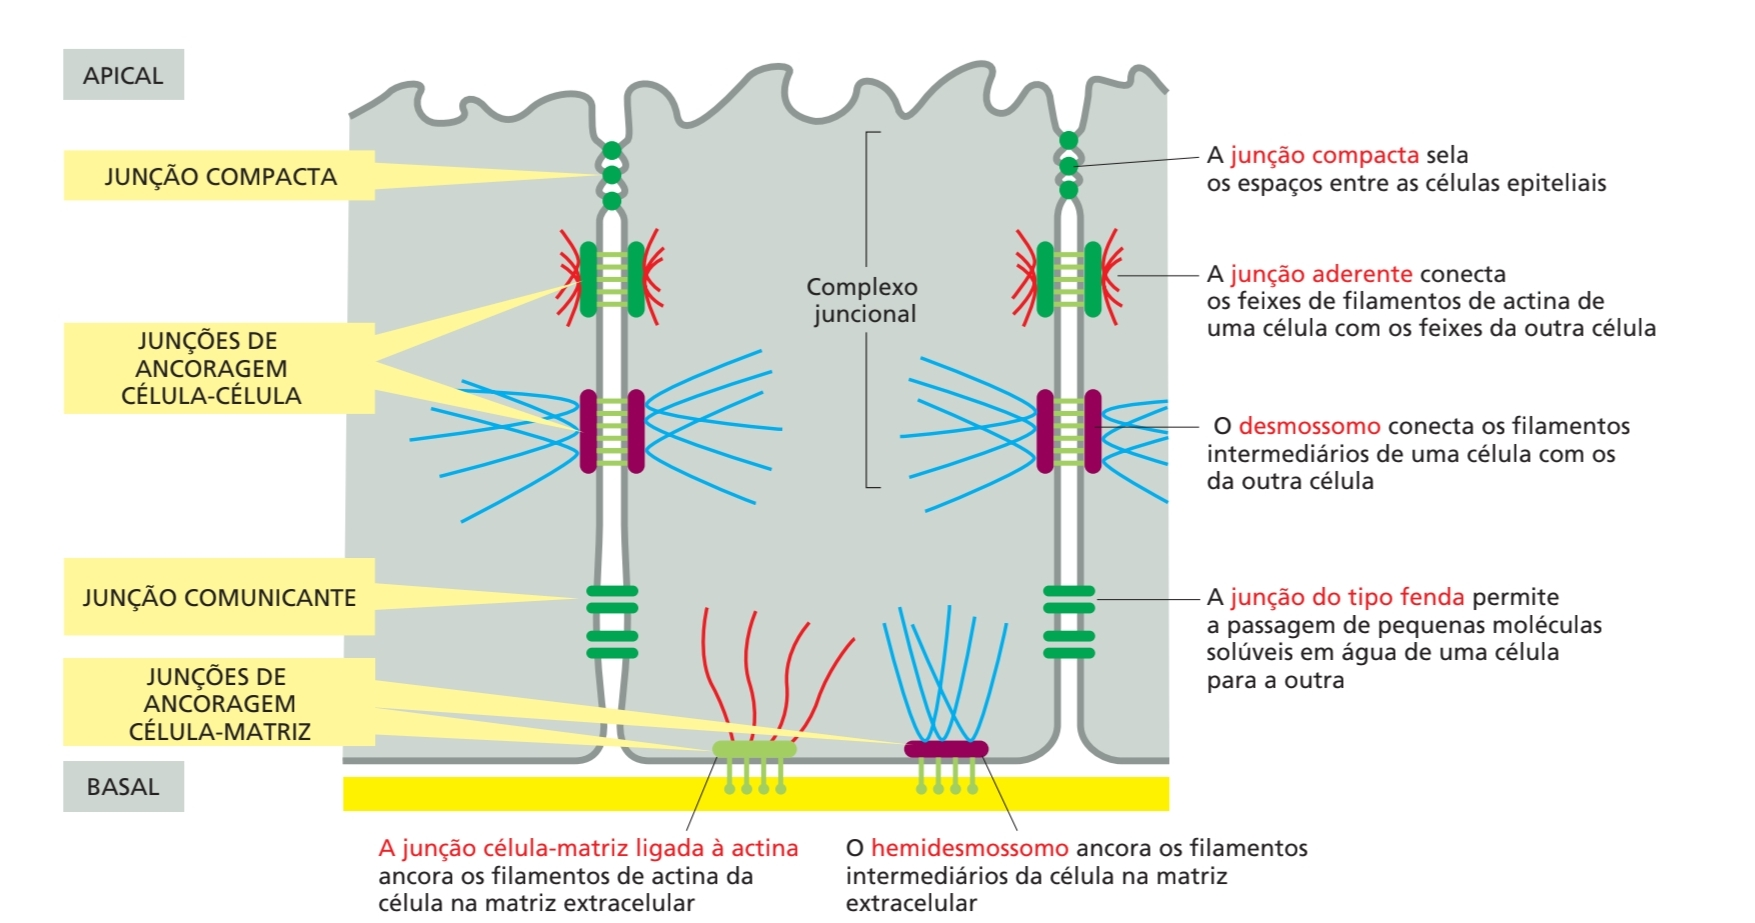
\includegraphics[width=0.8\textwidth]{img/bio/celula_celula.jpg}
        \caption{Tipos de ligação célula-célula}
    \end{figure}
\end{frame}

\section{Influência das Barreiras de Energia nas Intreações Moleculares}
\begin{frame}{Barreias de Energia}
Os processos de ligações são dinâmicos. Como mencionado, as ligações são não covalentes e
têm diversas forças envolvidas, entre elas:
\begin{itemize}
    \item Repulsão de Van de Waals
    \item Atração de Lonodon (interações de dipolo)
    \item Coloumbiana (atrativa e repulsiva)
\end{itemize}
Todas as forças dependem da torção, flexão e alongamento das ligações químicas.
\end{frame}

\begin{frame}
    \begin{figure}\label{fig:barreiras-energia}
        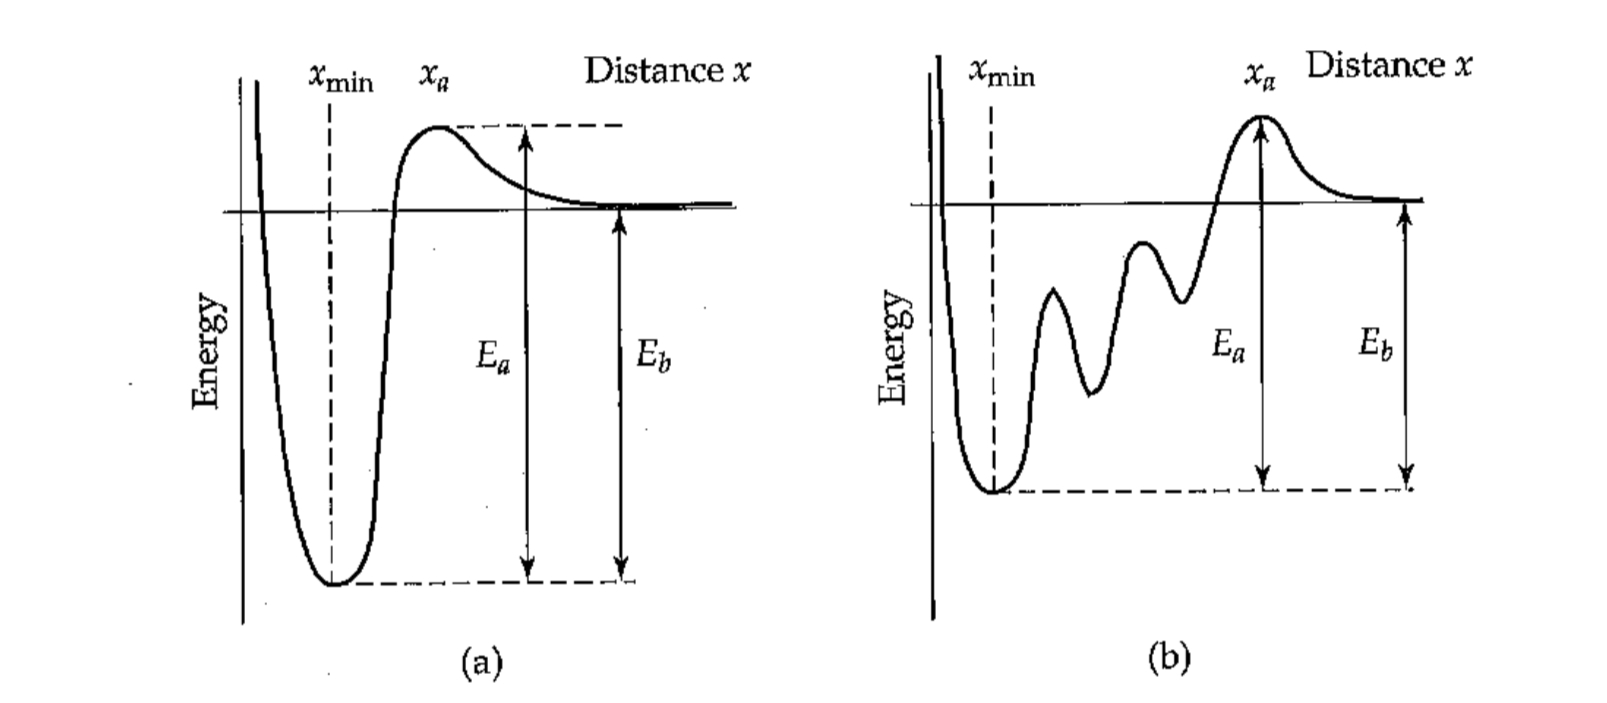
\includegraphics[width=0.8\textwidth]{img/barreiras_energia.jpg}
        \caption{(a) Interações moleculares simples (b) Múltiplas interações moleculares}
    \end{figure}    
\end{frame}

\begin{frame}{Taxa de Dissosiação}
    Quando se trata de energias, temos que analisar a taxa de formação e dissociação.
    De forma macroscópica podemos de forma geral escrever como:
    \begin{equation}
    k_{-1} = \nu \exp \left( \frac{E_{a}}{k_{b} T}\right) \label{eq:disso-k}
    \end{equation}
    em que $\nu$ é um prefator, $E_{a}$ a energia de ativação para quebrar a ligação, $k_{B}$
    é a constante de Boltzman e $T$ a temperatura absoluta.
\end{frame}

\begin{frame}{Taxa de Dissosiação}
    \begin{figure}
        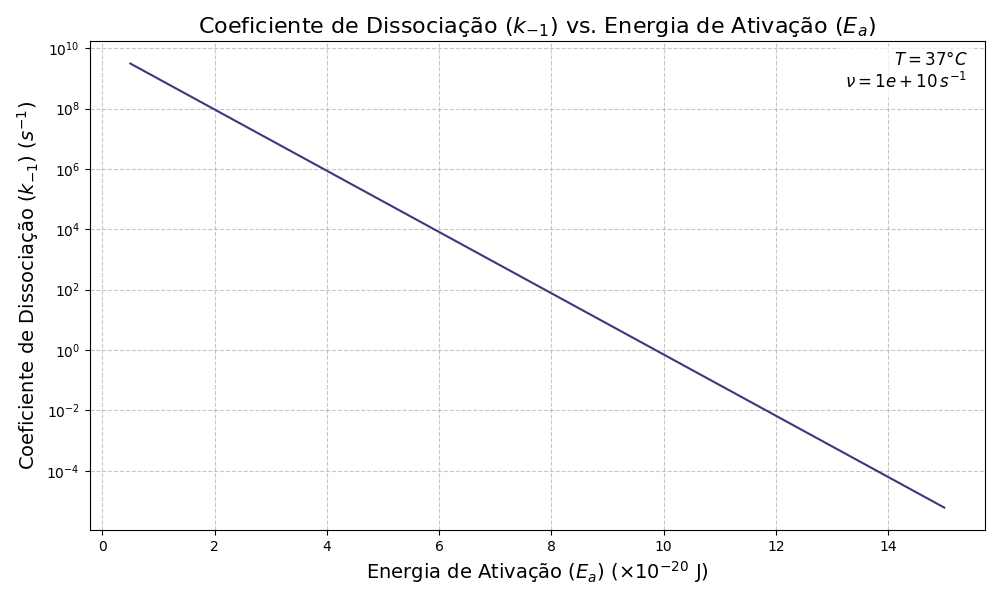
\includegraphics[width=0.7\textwidth]{img/coef_diss_energia.png}
        \caption{Plot de valores de energia de relacionados com o coeficiente}
    \end{figure}
\end{frame}

\begin{frame}{Taxa de Dissosiação}
    \begin{figure}
        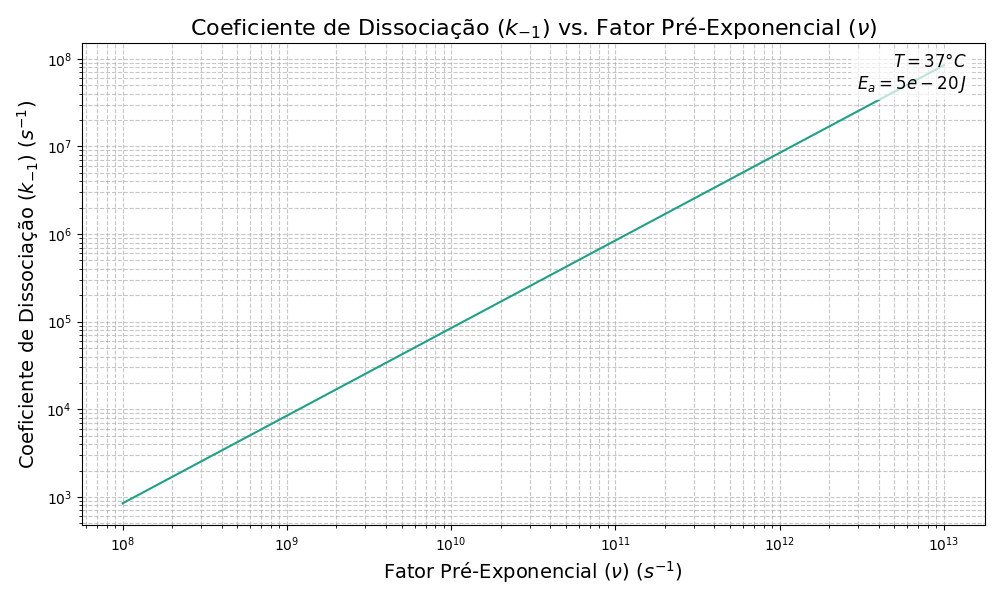
\includegraphics[width=0.7\textwidth]{img/coef_diss_fatorpre.png}
        \caption{Plot de valores variando o fator pré-exponencial}
    \end{figure}
\end{frame}

\begin{frame}{Probabilidade de Dissosiação}
    Conectando com a equação\eqref{eq:disso-k}, podemos construir uma probabilidade de uma ligação dissociar
    \begin{equation}
        p = 1 - \exp (-k_{-1} t)
    \end{equation}
\end{frame}

\begin{frame}{Probabilidade de Dissosiação}
    Podemos variar os parâmetros para visualizar o comportamento das ligações
    \begin{figure}
        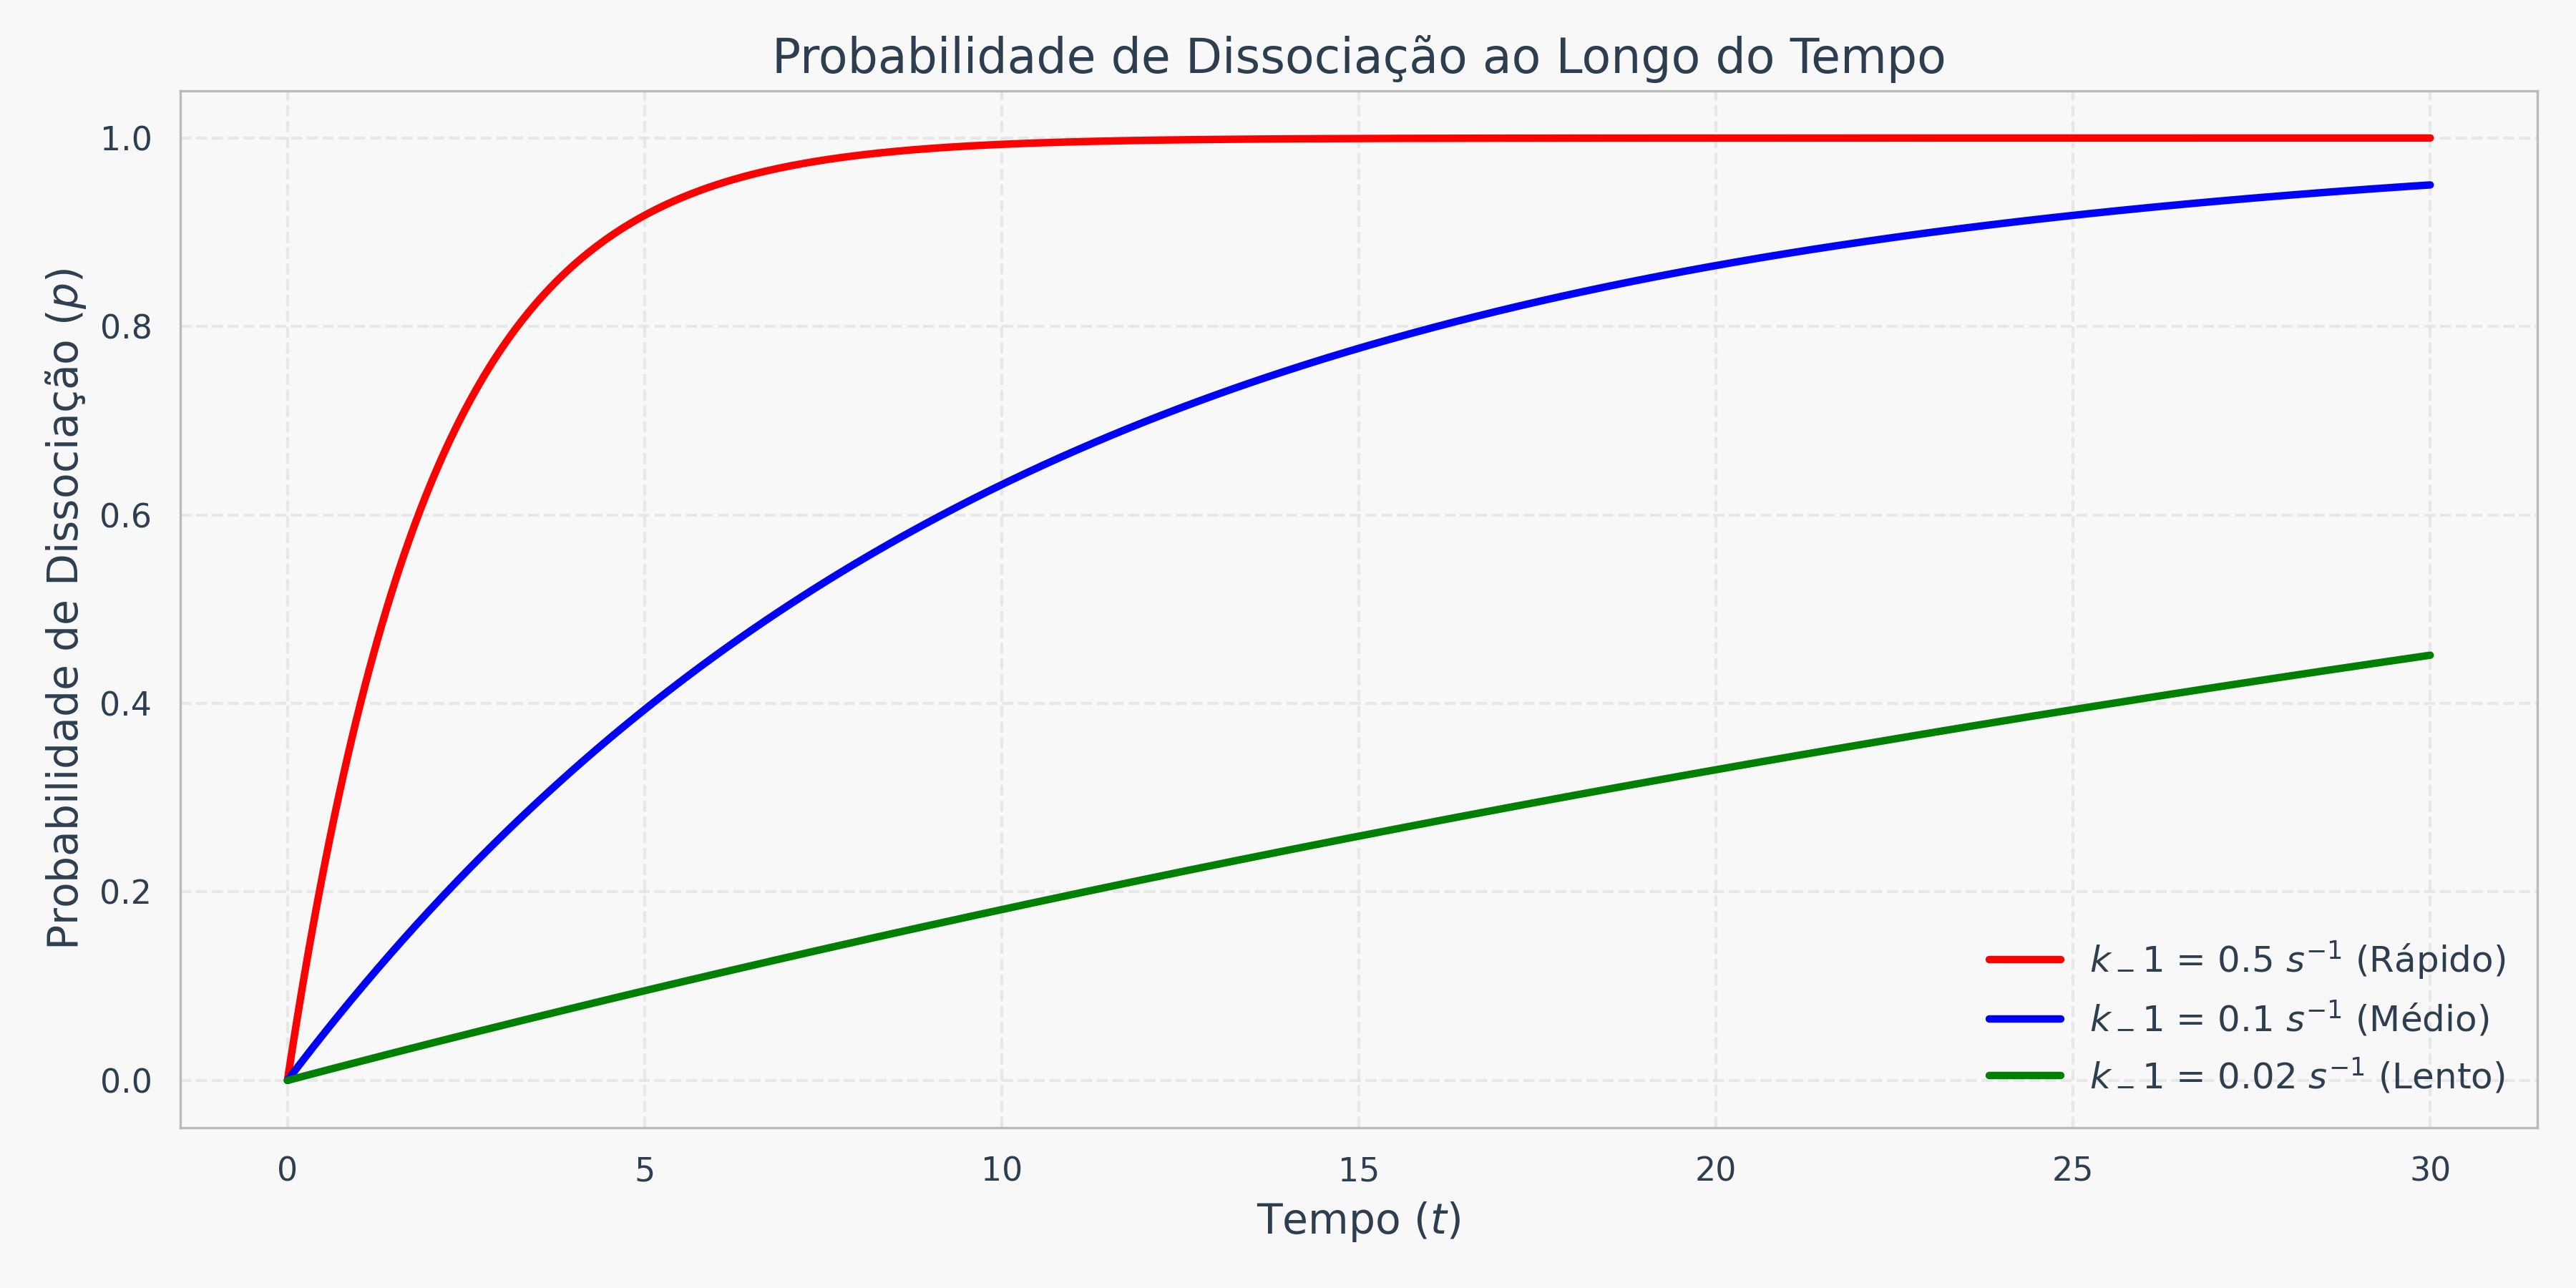
\includegraphics[width=0.7\textwidth]{img/prob_diss_tempo.png}
        \caption{Teste com 3 valores de $k_{-1}$}
    \end{figure}
\end{frame}

\section{Dissociação na Presença de Forças}

\begin{frame}{Taxa de Dissociação Forçada}
    Quando uma força $F$ é aplicada, esperamos a barreira de energia mudar um $\delta E_{a}$,
    fazendo com que a dissociação seja facilitada. Matematicamente, Bell postulou uma mudança $x_{a}F$,
    com isso, a equação\eqref{eq:disso-k} se torna:
    \begin{equation}
        k_{-1} = \nu \exp \left( \frac{E_{a} - x_{a}F}{k_{b} T} \right)
    \end{equation}
    ou, colocando em evidência uma taxa sem estresse $k_{-1}^{0}$
    \begin{equation}\label{eq:stressed-disso-k}
        k_{-1} = k_{-1}^{0} \exp \left( \frac{x_{a}F}{k_{b} T} \right)
    \end{equation}
\end{frame}

\begin{frame}{Modelo de Hooke}
    Uma forma mais explícita de lidar com a força é usando a Lei de Hooke $F = \kappa (x - x_{min})$.
    Usamos a descrição termodinâmica para a constante de equilíbrio
    \begin{equation}
        K_D = \exp \left(\frac{\Delta G}{k_B T} \right)
    \end{equation}
    aplicando a Lei de Hooke
    \begin{equation}
        K_{D} = K_{D}^{0} \exp \left[\frac{0.5 \kappa (x-x_{\min})^2}{k_{B} T}\right]
    \end{equation}
\end{frame}

\begin{frame}{Modelo de Hooke}
    Com essa equação em mãos, podemos analisar a taxa de dissosiação
    \begin{equation}\label{eq:disso-k-hooke}
        k_{-1} = k_{-1}^{0} \exp \left[\frac{\kappa (x_{a} - x_{\min})(x-x_{\min})}{k_{B} T}\right]
    \end{equation}
\end{frame}

\begin{frame}{Modelo de Hooke}
    \begin{figure}
        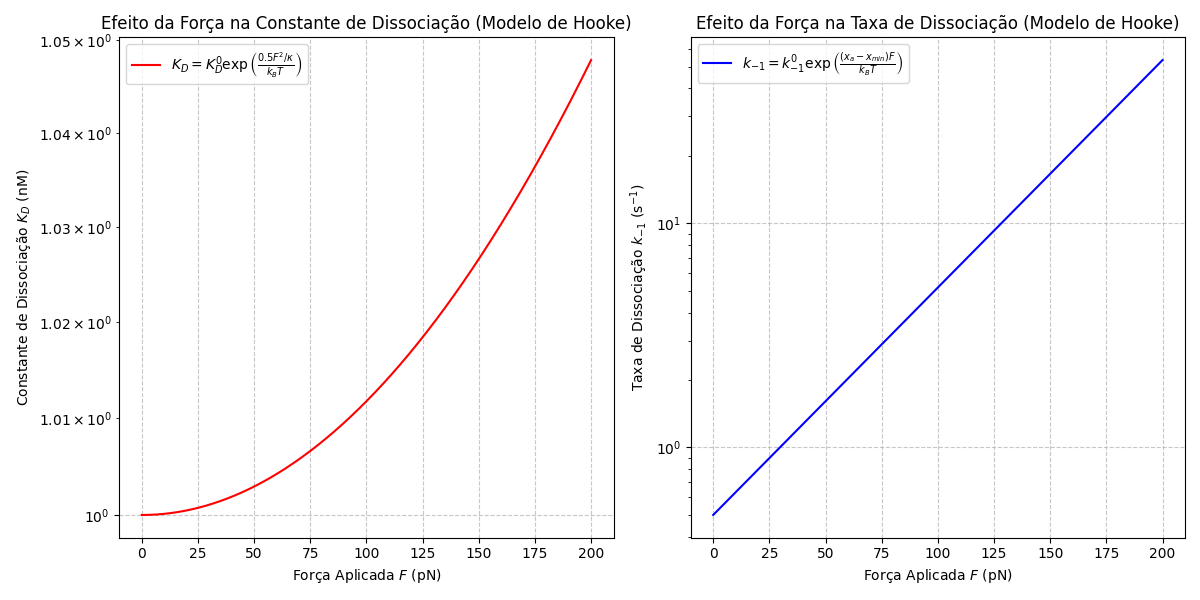
\includegraphics[width=0.8\textwidth]{img/coef_diss_hooke.png}
        \caption{Análise de $K_D$ e $k_{-1}$}
    \end{figure}
\end{frame}

\begin{frame}{Efeitos de Forças Variáveis}
    As equações anteriores mostram modelos quando uma força em específica é atuada em todo o sistema
    de forma direta e sem variações. Em uma célula, colisões, principalmente de moléculas de água mudam
    a dinâmica das ligações. Diversos trabalhos experimentais foram desenvolvidos para categorizar
    essas forças. Com isso, foi encontrado a seguinte relação para calcular a força necessária para dissociação:
    \begin{equation}
        F_{b} = \frac{k_{b} T}{x_{a}} \ln \left(\frac{r_{f} x_{a}}{k_{-1}^{0} k_{B} T}\right)
    \end{equation}
    Em que $r_{f}$ é chamado de \textit{loading rate}
\end{frame}

\section{Adesão Celular à Matriz Extracelular}

\begin{frame}{Anexo entre células}
    O processo de adesão é separado em duas fases: ligação e desprendimento. Para a ligação, temos
    que relacionar três variáveis de ligação
    \begin{itemize}
        \item $N_{C}$: Número de complexos ligantes \textbf{ligados} na membrana
        \item $N_{L}$: Número de complexos ligantes \textbf{não ligados} na membrana
        \item $N_{R}$: Número de receptores \textbf{não ligados}
    \end{itemize}
    Com isso, temos a equação
    \begin{equation}\label{eq:var_receptores}
        \frac{d N_C}{dt} = k'_{1} N_{L} N_{R} - k_{-1}N_{C}
    \end{equation}
\end{frame}

\begin{frame}{Anexo entre células}
    Considerando constante o número total de cada tipo de moléculas:
        \begin{align}\label{eq:lig_constante}
            N_{L_0} &= N_L + N_C \\
            N_{R_0} &= N_R + N_C 
        \end{align}
    Substituindo, temos
    \begin{equation}
        \frac{d N_C}{dt} = k'_{1} (N_{L_0} - N_C) (N_{R_0} - N_C) - k_{-1}N_{C} \label{eq:lig_geral}
    \end{equation}
\end{frame}

\begin{frame}{Anexo entre células}
    Resolvendo a equação \eqref{eq:lig_geral}, obtemos:
    \begin{equation}
        N_C = \frac{b+\sqrt{b^2-4a}}{2}\left\{\frac{1-\exp[-k_1 (\sqrt{b^2-4a})t]}{1-\left(\frac{b+\sqrt{b^2-4a}}{b-\sqrt{b^2-4a}}\right)\exp[-k_1 (\sqrt{b^2-4a})t]}\right\}
    \end{equation}
    Onde os termos $a$ e $b$ são definidos como:
        \begin{align*}
            a &= N_{L_0}N_{R_0} \\
            b &= N_{L_0} + N_{R_0} + K_D
        \end{align*}
\end{frame}

\begin{frame}{Desprendimento de Células}
    Como as superfícies das céluas têm receptores distribuídos de forma heterogênea, para desprender
    duas células, é necessário aplicar uma quantidade de força no tempo. De forma experimental, foi mostrada
    que essa força é descrita como:
    \begin{equation}
        f(\tau_{\omega}, t) = 1 - \int_0^{\tau_{\omega}} p(\mu, \sigma, \tau) d\tau
    \end{equation}
    em que $p(\mu, \sigma, \tau)$ é uma distribuição lognormal e $\tau$ é uma tensão de cisalhamento.
    \begin{equation}
        p(\mu_{x}, \sigma_{x}, \tau) = \frac{1}{\tau \sigma \sqrt{2 \pi}} \exp \left( - \frac{(\ln \tau - \mu)^{2}}{2 \sigma^{2}} \right)
    \end{equation}
\end{frame}

\begin{frame}
    \begin{figure}
        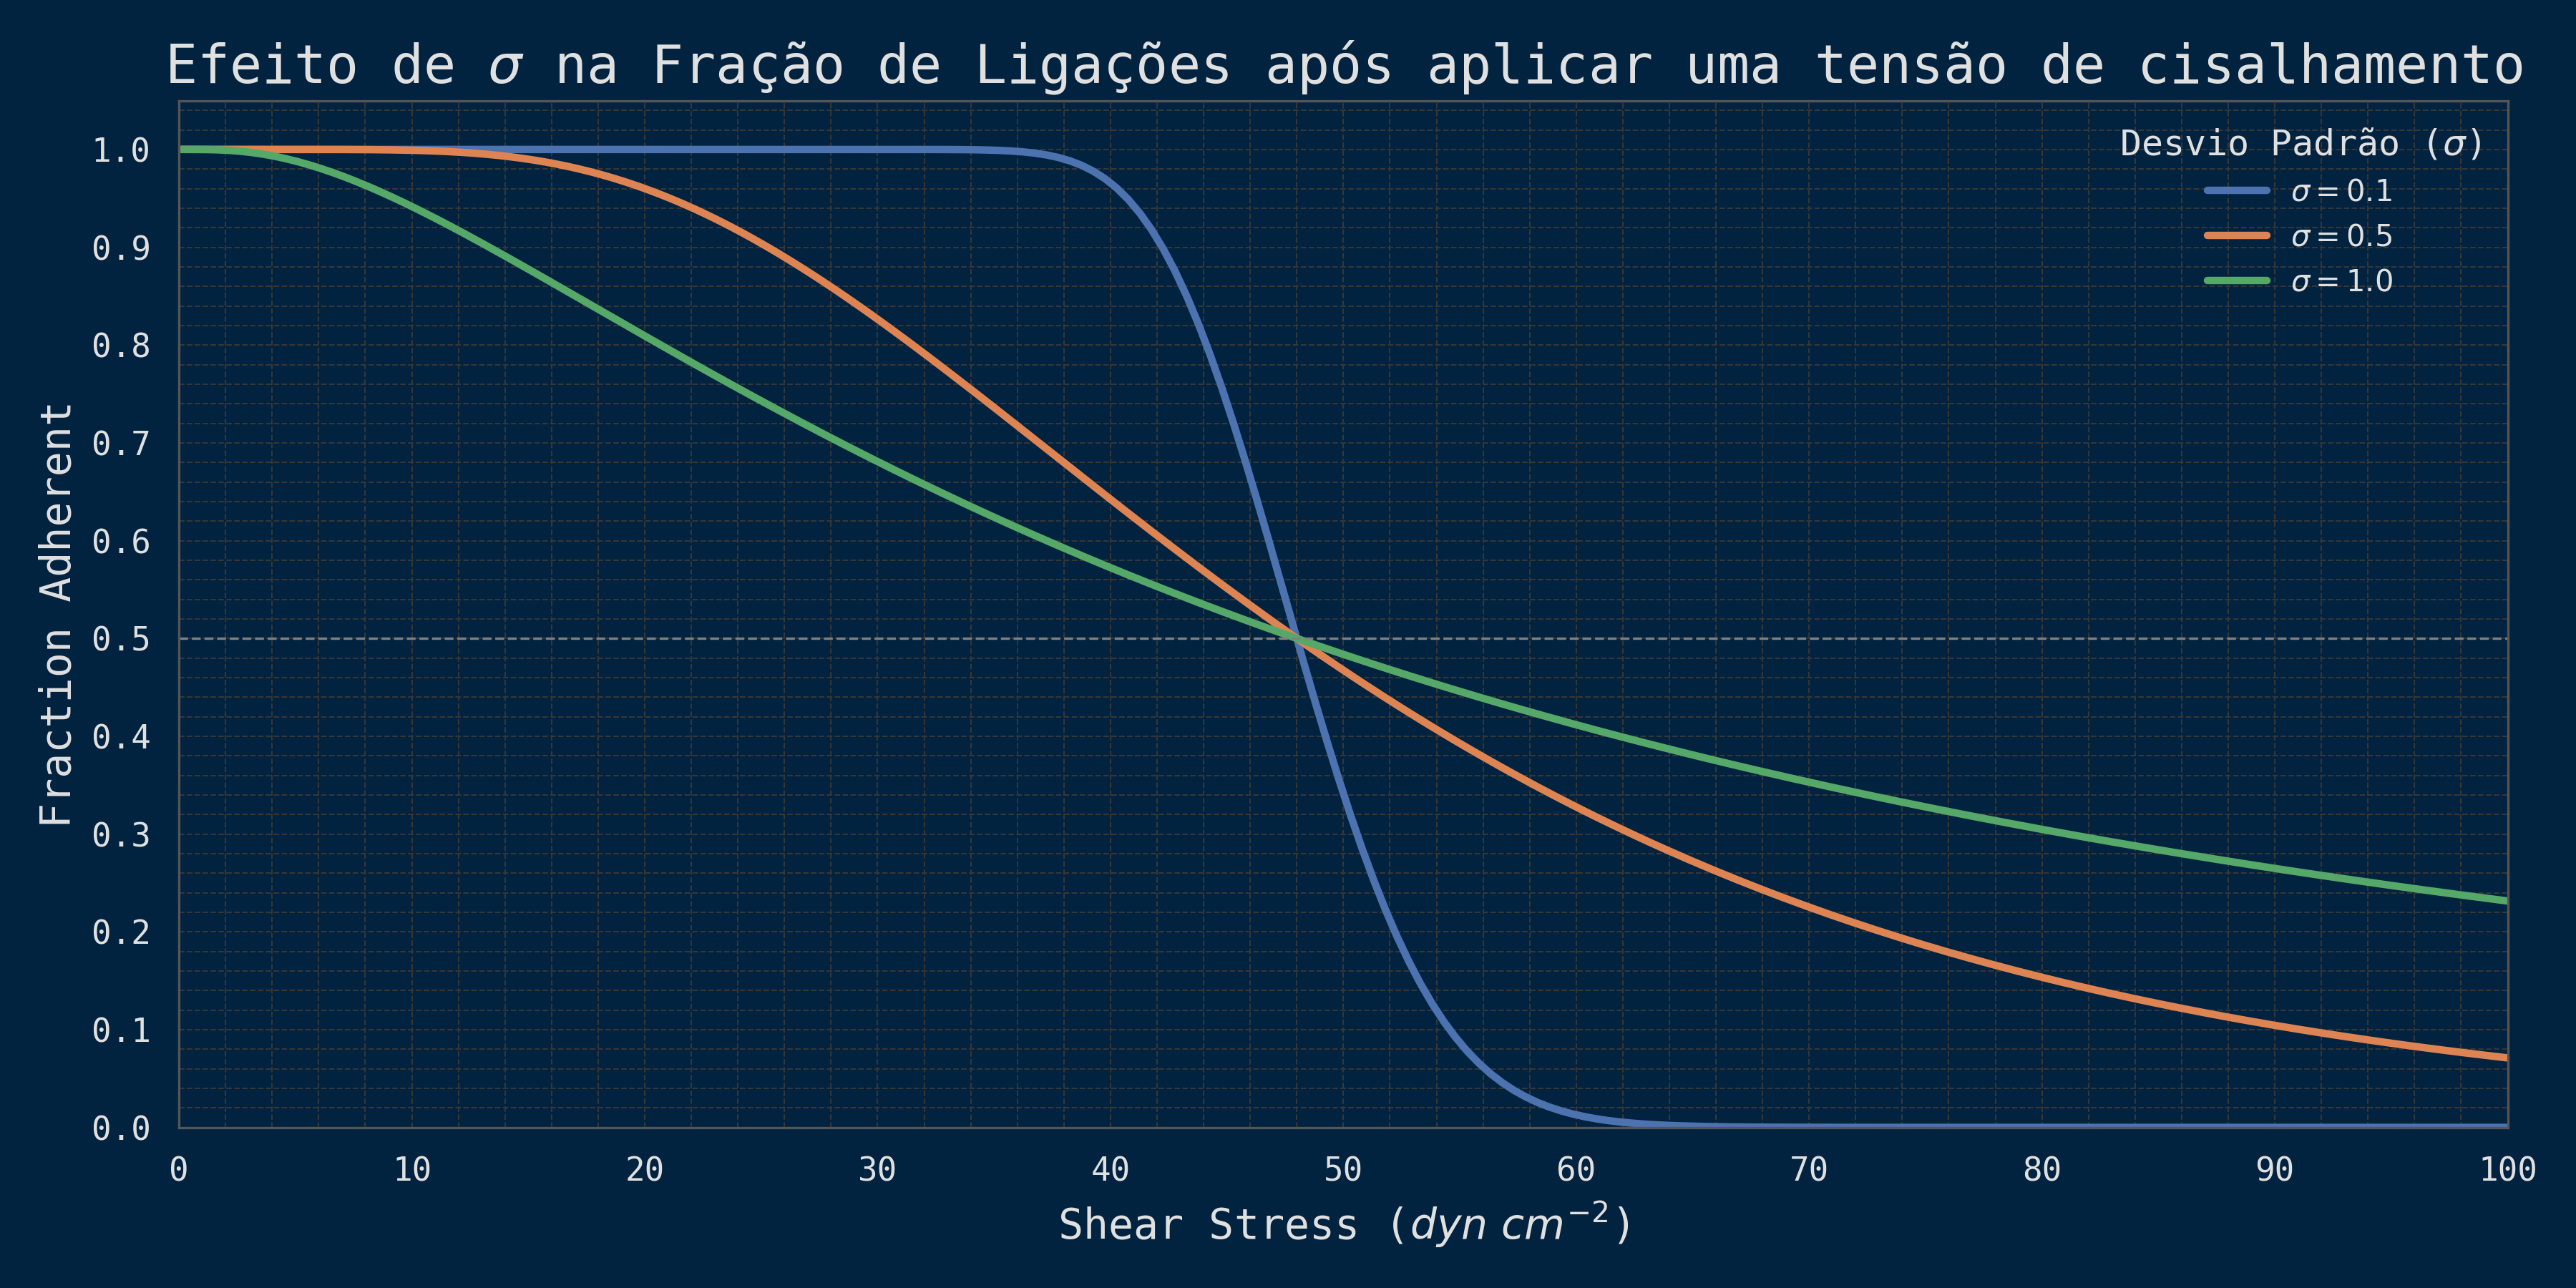
\includegraphics[width=0.8\textwidth]{img/sigma_cisalhamento.png}
        \caption{Variação do parâmetro sigma}
    \end{figure}
\end{frame}

\begin{frame}{Desprendimento de células}
    Com esses resultados, podemos calcular numericamente usando a equação de Navier-Stokes ou Stokes, caso o número de Reynolds for menor que 0,1.
    Para células esféricas, apenas tocando a superfície, a força de arrasto e momento:
    \begin{align}
        F_D &= 6 \pi \dot{\gamma} \mu a h F_{x}\left(\frac{a}{h}\right) \\
        T &= 4 \pi \dot{\gamma} \mu a^{3} M_{z} \left(\frac{a}{h}\right)
    \end{align}
    De forma numérica, foi calculado usando a equação de Stokes:
    \begin{align}
        F_D &= 4.50 \pi \dot{\gamma} \mu a^{2} \\
        T &= 2.58 \pi \dot{\gamma} \mu a^{3}    
    \end{align}
\end{frame}

\begin{frame}{Desprendimento de células quando há forças}
    Quando uma célula é exposta a um fluxo, as equações que descrevem as ligações são sensíveis à interação hidrodinâmica.
    Então, podemos escrever a variação das ligações da seguinte forma:
    \begin{equation}
        \frac{d N_C}{dt} = k_{1}(N_{L_0} - N_C)(N_{R_0} - N_C) - k_{-1}^{0} \exp \left(\frac{x_a F}{k_b T N_C} \right) N_C
    \end{equation}
    Fazendo as substituições:
    \begin{itemize}
        \item $\tau = k_1 N_{L_0} t$
        \item $\kappa = \frac{K^{0}_{D}}{N_{L_0}}$
        \item $\alpha = \frac{x_a F}{k_B T N_{R_0}}$
        \item $\theta = \frac{N_C}{N_{R_0}}$
    \end{itemize}

\end{frame}

\begin{frame}
    As equações se tornam:
    \begin{equation}
        \frac{d \theta}{d \tau} = 1 - \theta - \kappa \theta \exp \left(\frac{\alpha}{\theta}\right)
    \end{equation}

    \begin{figure}
        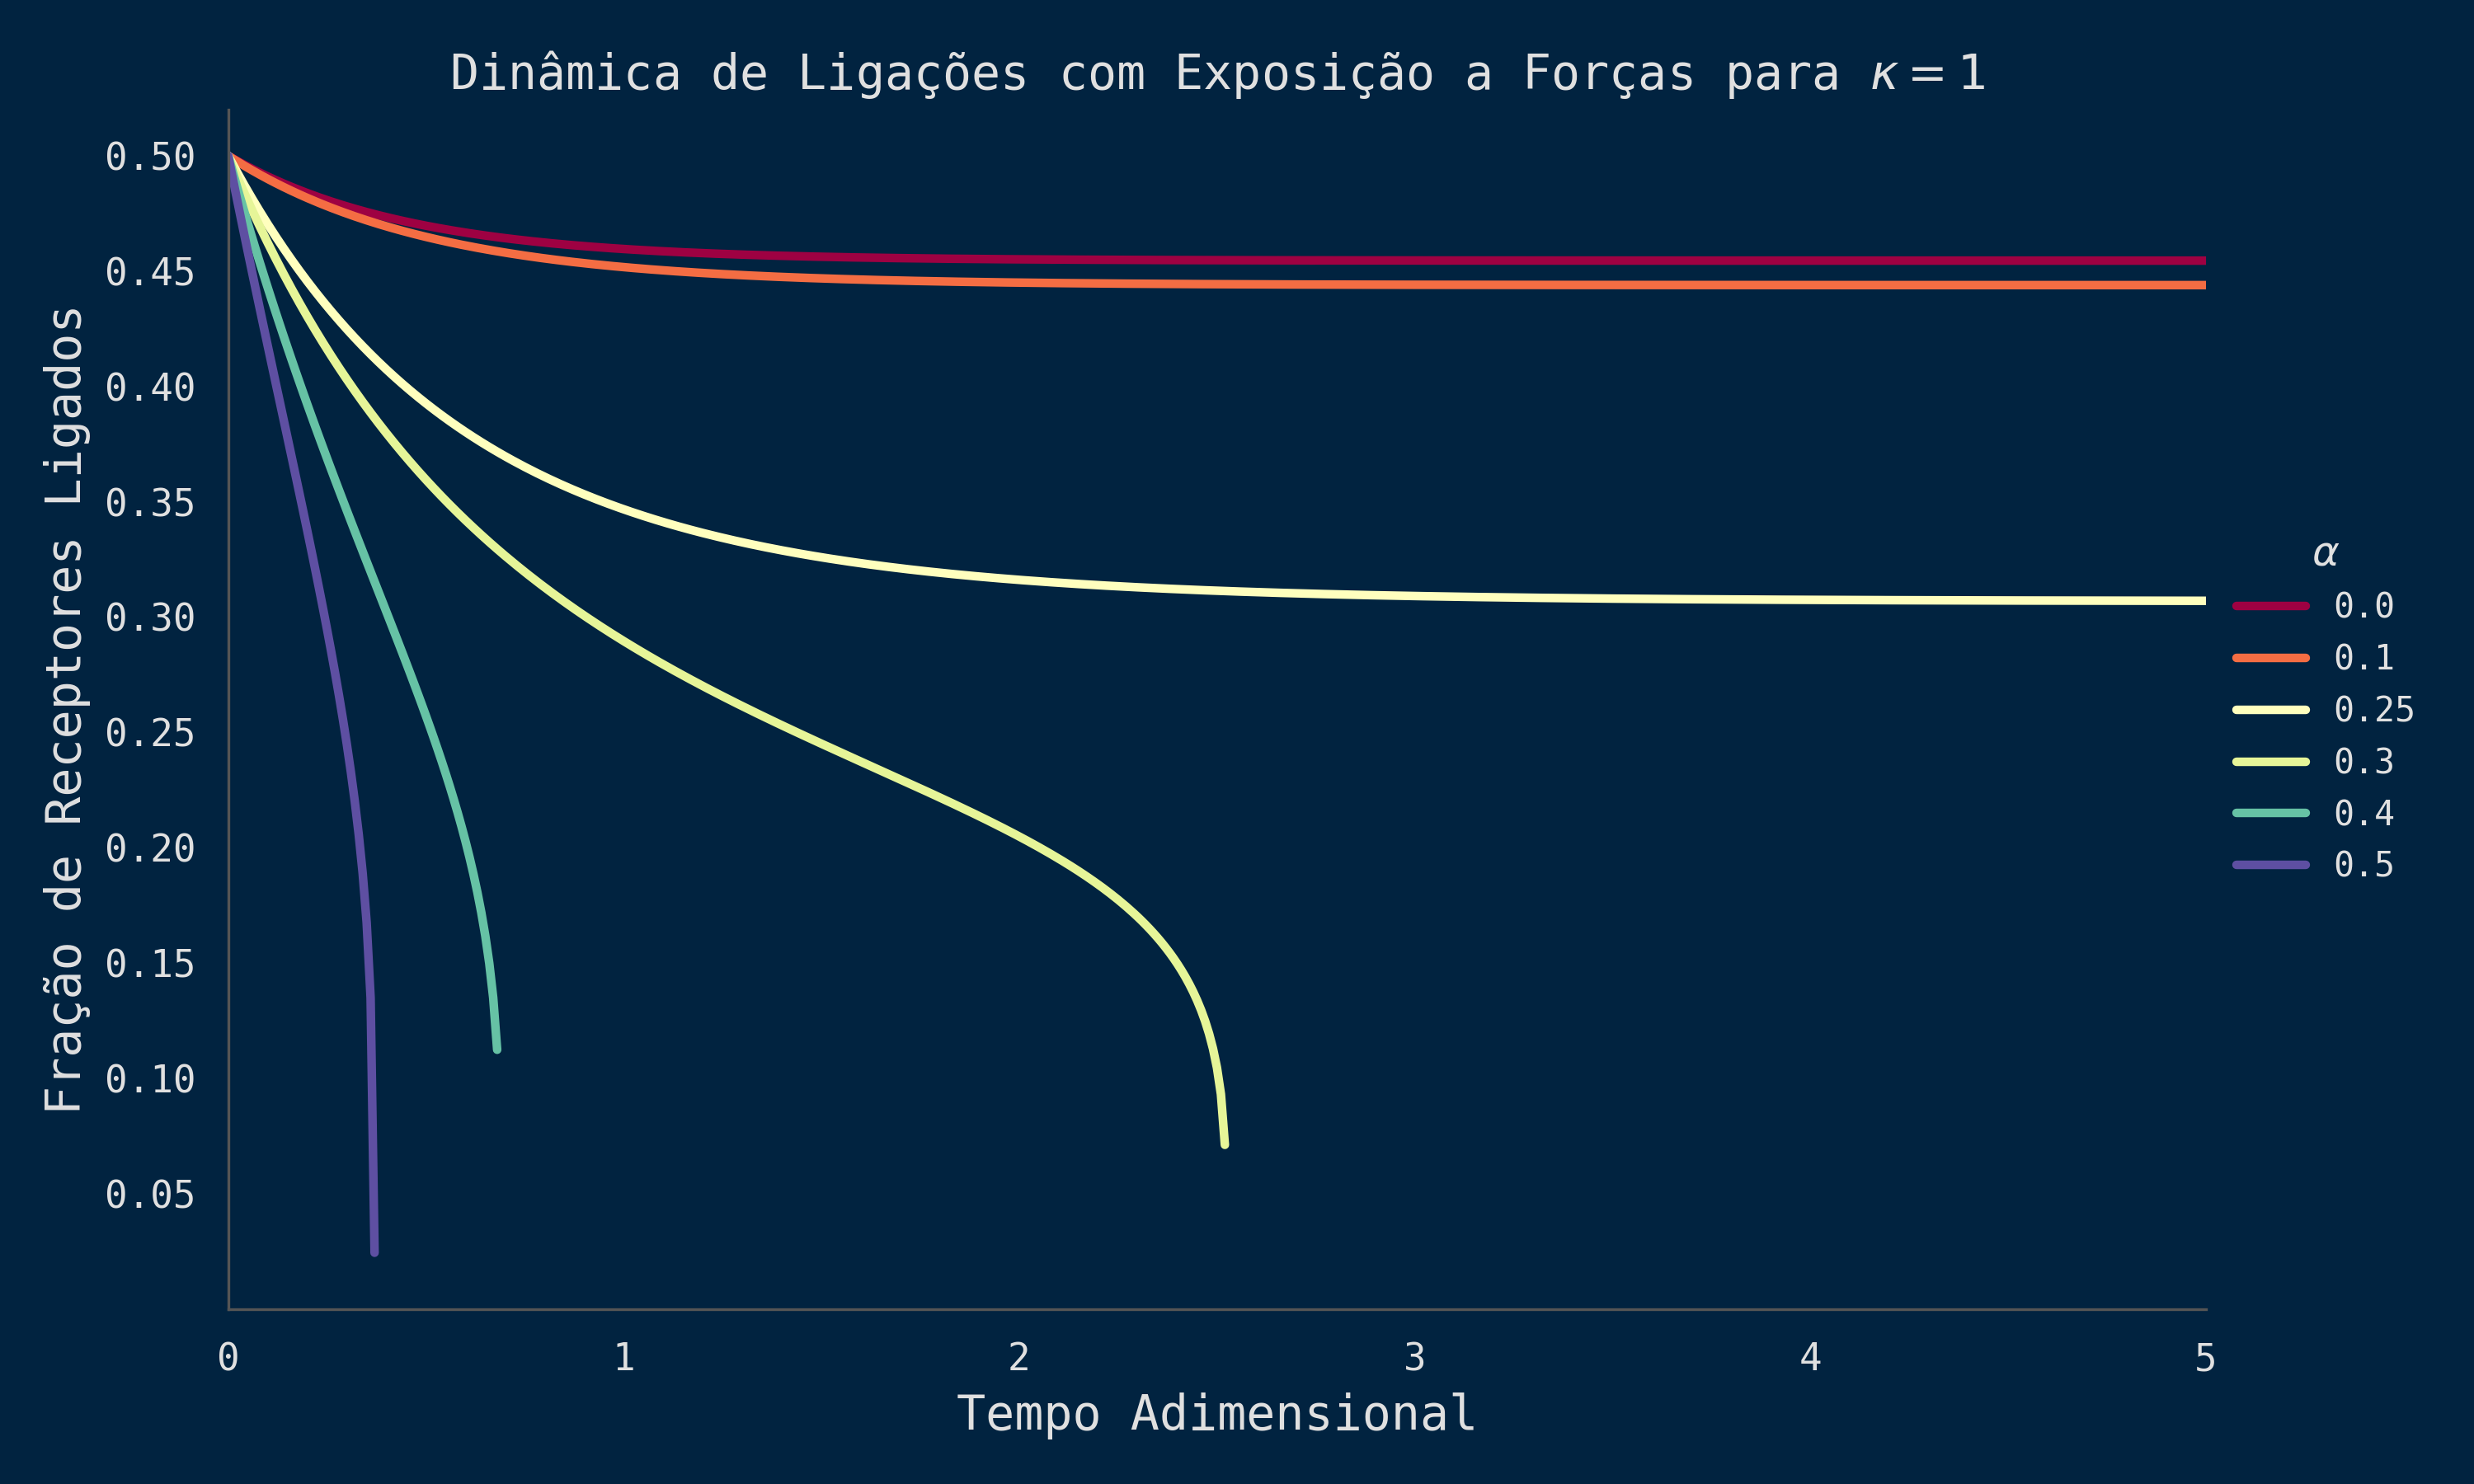
\includegraphics[width=0.6 \textwidth]{img/dettach_force.png}
    \end{figure}

\end{frame}

\section{Biofísica de Leucócitos Rolando e Aderindo}

\begin{frame}
    Para leucócitos, temos que ter em mente que todo esse processo é estocástico, temos que formar números
    de ligações e dissociar ligações dependendo da força gerada durante o movimento.
    Para esse caso, a probabilidade de formação de ligações deve ser dinâmica e considerar todas as interações, para um espaço de tempo curto e poucas ligações:
    \begin{equation}
        \frac{d P_{i}}{dt} = k_{ad} P_{i-1} + (i+1)k_{r}^{i+1}P_{i+1} - (k_{ad} + i k_{r}^{i}) P_{i}
    \end{equation}
    em que
    \begin{equation}
        \frac{dP_{0}}{dt} = (k_{r}^{1} - k_{ad}) P_{1}
    \end{equation}
    
    e
    \begin{equation}
        \frac{d P_{n}}{dt} = k_{ad} P_{n-1} - (k_{ad} + n k^{n}_{r}) P_n      
    \end{equation}
\end{frame}

\end{document}
